% !TeX encoding = windows-1251
\documentclass[12pt,a4paper]{article}
\usepackage[mag=1000]{newlistok}
\usepackage{tikz}\usetikzlibrary{calc, patterns}

\УвеличитьШирину{1cm}
\УвеличитьВысоту{1.9cm}
\renewcommand{\spacer}{\vspace{2.5pt}}


\begin{document}

\Заголовок{Разбиение на пары}
\НадНомеромЛистка{179 школа, 7Б.}
\НомерЛистка{5}
\ДатаЛистка{20.09 -- 30.09 /2017}
\СоздатьЗаголовок
\smallskip

{
%\footnotesize
\small

Часто в повседневной жизни нам приходится сравнивать количества различных объектов.
Во многих случаях нас интересует не сами количества, а ответ на вопрос: каких из них больше?
Так, при игре в слова победителем считается тот, кто придумал больше слов.
Поэтому при подведении итогов совсем не обязательно считать количество слов каждого, достаточно как-то придумать, как сравнить эти количества.
Приведём несколько примеров, как можно проводить такие сравнения без всяких подсчётов и вычислений.
\пример
Предположим, что воспитатель детского сада во время утренней прогулки решил выяснить, кого у него в группе больше: мальчиков или девочек.
Посчитать их явно довольно сложно, поскольку они всё время двигаются и есть опасность кого-то посчитать два раза, а кого-то пропустить.
Наверное одним из самых простых выходов в данной ситуации будет предложить детям построиться парами мальчик-девочка.
Если у них это получится, то мальчиков и девочек в группе поровну.
Если же какие-то мальчики окажутся без пары, то мальчиков больше. В противном же случае больше девочек.
\кпример

\пример
Петя и Вася решили выяснить, кто из них может сделать больше приседаний.
Считать сначала, сколько может присесть первый, а потом второй, им не подходит, поскольку после двух десятков приседаний они боятся сбиться со счета и ошибиться.
Поэтому можно предложить им начать приседать одновременно и делать приседания синхронно (т.е. тоже одновременно).
В этом случае тот, кто первый не сможет больше приседать, и будет проигравшим.
\кпример

\пример
Пусть в зале собралось некоторое количество людей, и мы хотим установить, хватит ли на них на всех стульев (или надо принести ещё).
То есть нужно сравнить количество людей и количество стульев.
Можно конечно попытаться пересчитать и людей, и стулья.
Но люди постоянно перемещаются, некоторые стулья мы можем не заметить, да и пересчитывая большое количество стульев легко ошибиться.
Вместо этого предложим всем людям сесть на стулья.
Если все люди сумели сесть и свободных стульев при этом не осталось, то количество людей равно количеству стульев.
Если же, к примеру, окажется, что все стулья заняты, а кто-то всё ещё продолжает стоять, то стульев меньше, чем людей.
\кпример

Во всех трёх примерах мы делали однотипную операцию, и вот её математическая формулировка:

\опр
Говорят, что между двумя множествами установлено \выд{взаимно-однозначное соответствие} (или \выд{биекция}),
если любому элементу (объекту) первого множества соответствует единственный элемент (объект) второго множества и наоборот.
\копр

В первом примере мы рассматривали множество мальчиков и множество девочек.
Строя их парами мальчик-девочка, мы пытались установить взаимно-однозначное соответствие между множеством мальчиков и множеством девочек.
Во втором примере первое множество состояло из отдельных приседаний Пети, а второе — из отдельных приседаний Васи.
После этого мы пытались сравнить количество отдельных приседаний в первом множестве и во втором, чтоб определить победителя.
Для этого мы первому приседанию Пети ставили в соответствие первое приседание Васи, второму приседанию Пети — второе приседание Васи и т.д.
Тем самым мы пытались установить биекцию между этими двумя множествами.
В третьем примере мы пробовали установить биекцию между множеством людей и множеством стульев.
Если бы все стулья оказались заняты людьми, а часть людей ещё продолжала бы стоять,
то нам удалось установить взаимно-однозначное соответствие между множеством стульев и частью множества людей.
Все сказанное выше позволяет сделать три очевидных утверждения:

\утв
Если имеются два конечных множества $A$ и $B$ с одинаковым количеством элементов,
то между ними можно установить взаимно-однозначное соответствие, разбив их на пары:
первому элементу множества $A$ можно поставить в соответствие первый элемент множества $B$,
второму элементу множества $A$ — второй элемент множества $B$ и т.д.
\кутв

\утв[обратное]
Если между двумя конечными множествами можно установить взаимно-однознач\-ное соответствие, то в них одинаковое количество элементов.
\кутв

\утв
Если между конечным множеством $A$ и частью конечного множества $B$ можно установить взаимно-однозначное соответствие,
то в множестве $B$ больше элементов, чем в множестве $A$.
\кутв

В отличие от реальных людей, которые сами находить себе стулья, в математических задачах объекты не смогут сами разбиться на пары без нашего участия и чёткого описания, какому объекту какой соответствует.
Поэтому решение математических задач, в которых устанавливается биекция, должно состоять из трёх этапов.
Если эти этапы перевести на язык людей и стульев, то они выглядят следующим образом:
\begin{nums}{-3}
\item Указать, какому человеку на какой стул садиться.
\item Проверить, что разные люди при этом должны будут сесть на разные стулья, т.е. убедиться, что нескольким людям не указано на один и тот же стул.
\item Выяснить, для каждого ли стула есть человек, который должен на него сесть
\end{nums}


} % конец small-а

\newpage






















\smallskip
\задача
На окружности нарисованы 10 чёрных точек и одна
белая. Чего больше: треугольников,
все вершины которых чёрные, или четырёхугольников с
тремя чёрными вершинами и одной белой?
\кзадача

\пзадача
Все последовательности из 20 нулей и единиц делятся
на две группы --- те, в которых чётное число единиц, и те,
в которых нечётное. Каких больше?
\кзадача

\пзадача
Некоторое число делится на $2$, но не делится на $4$. Докажите, что
количество ч\"етных делителей этого числа равно количеству
его неч\"етных делителей.
\кзадача

\пзадача
Докажите, что натуральное число имеет нечётное число натуральных делителей тогда и только тогда,
когда оно является точным квадратом.
\кзадача

\пзадача
Назовём число <<убывающим>>, если цифры в его записи убывают, и <<возрастающим>> --- если возрастают.
\пункт Каких <<убывающих>> чисел больше --- трёхзначных или семизначных?
\пункт Каких <<возрастающих>> чисел больше --- трёхзначных или семизначных?
\кзадача

\пзадача
Почему число решений уравнения $x+y+z = 30$ в положительных целых числах равно числу решений уравнения
$x + y + z = 27$ в неотрицательных целых числах?
\кзадача

\пзадача
Петя выписал на доску все тройки целых чисел $(x;y;z)$, для которых $0<x<y<z<13$.
Вася выписал на доску все тройки целых чисел $(a;b;c)$, для которых $0\leq a\leq b\leq c\leq9$.
У кого получилось больше троек?
\кзадача

\задача
Среди треугольников с целыми сторонами
каких больше:\\
%\вСтрочку
\пункт
периметра 2014 или периметра 2017;
\пункт
периметра 2015 или периметра 2018?
%с целыми сторонами
\кзадача


% \сзадача
% Докажите, что число разбиений выпуклого $n$-угольника на
% треугольники непересекающимися диагоналями равно числу способов расстановки скобок в произведении $n - 1$ сомножителей.
% \кзадача

\сзадача
Петя подсчитал количество всевозможных $m$-буквенных слов, в записи которых могут использоваться только буквы {\it T}, {\it O}, {\it W} и {\it N}, причём в каждом слове букв {\it T} и {\it O} поровну. Вася подсчитал количество всевозможных $2m$-буквенных слов, в записи которых могут использоваться только буквы {\it T} и {\it O}, и в каждом слове этих букв поровну. У кого слов получилось больше?
(Слово --- это любая последовательность букв.)
\кзадача

\сзадача
Докажите, что число разбиений натурального $n$
на $k$ натуральных слагаемых равно числу разбиений $n$
в сумму натуральных слагаемых, наибольшее из которых равно $k$.
(Разбиения, отличающиеся лишь порядком слагаемых,
считаются~одинаковыми.)
\кзадача

% 10. Доказать, что количество разбиений целого положительного
% числа n на целые положительные слагаемые, не превосходящие k,
% равно количеству разбиений числа n на не более чем k целых по-
% ложительных слагаемых.

\сзадача
Докажите, что счастливых шестизначных номеров (то есть таких, где
сумма первых трёх цифр равна сумме трёх последних) столько же,
сколько шестизначных номеров с суммой цифр~27.
\кзадача


\сзадача
Докажите, что число способов разрезать доску $2\times (n+1)$ на доминошки равно числу последовательностей длины $n$ из нулей и единиц, в которых нет двух нулей подряд.
%(равно числу решений уравнения x_1+x_2+...+x_k=n таких, что всё x_i равны 1 или 2).
\кзадача

% \сзадача
% Докажите, что число разбиений натурального $n$
% на $k$ натуральных слагаемых равно числу разбиений $n$
% в сумму натуральных слагаемых, наибольшее из которых равно $k$.
% (Разбиения, отличающиеся лишь порядком слагаемых,
% считаются~одинаковыми.)
% \кзадача

\сзадача [Числа Каталана]
Докажите, что следующие величины совпадают:\\
$\bullet$
Число способов разрезать правильный $(n+2)$-угольник
на $n$ треугольников, проводя диагонали;\\
\centerline{
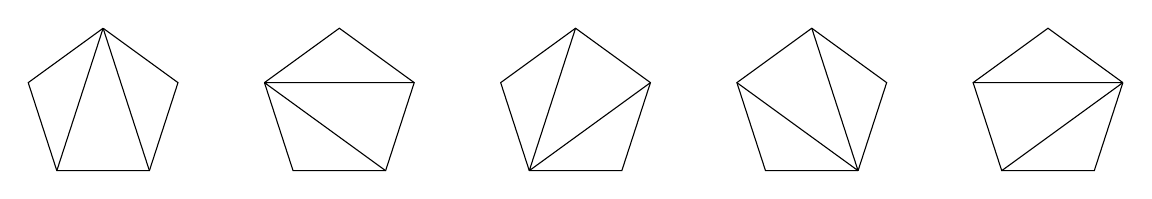
\begin{tikzpicture}
\foreach \shift/\rot in {0/0, 3/72, 6/144, 9/216, 12/288} {
\begin{scope}[xshift=\shift cm]\begin{scope}[rotate around={\rot:(0,0)}]
    \draw (90:1) \foreach \ang in {90,162,...,470} {--(\ang:1)};
    \draw (90:1) -- (234:1) (90:1)--(-54:1);
\end{scope}\end{scope}
}
\end{tikzpicture}}\\
\noindent
$\bullet$ Число способов расставить
скобки в произведении $n - 1$ сомножителей.\\ \\
%в ряд $n$ открывающих и $n$ закрывающих скобок;\\
{\hspace*{3cm}}\texttt{a(b(cd)) \ \ \ (ab)(cd) \ \ \ ((ab)c)d \ \ \ a((bc)d) \ \ \ (a(bc))d}
% $\bullet$ Число путей из точки $(0,0)$ в точку $(n,n)$, идущих по линиям
% клетчатой бумаги вверх и вправо, не поднимаясь
% выше прямой $y=x$;\\ \\ \\ \\ \\
% \rightpicture{-40mm}{20mm}{110mm}{cat-2}
% \vspace*{1cm}
%% \пункт Сколько существует последовательностей длины $2n$, в которых $n$ раз
%% встречается $1$, $n$ раз встречается $-1$, и все частичные
%% суммы (то есть суммы нескольких (одного, двух, тр\"ех, \dots) первых членов) %\footnote{$k$\д ой частичной суммой последовательности
%%%$a_1,\dots,a_p\ (k\le p)$ называется $a_1+\dots+a_k$}
%% неотрицательны?
%% \begin{center}
%% \texttt{
%% 1 1 1 {-1} {-1} {-1} \ \ \ 1 1 {-1} 1 {-1} {-1}\ \ \ 1 {-1} 1 1 {-1}
%% {-1}\ \ \ 1 {-1} 1 {-1} 1 {-1}\ \ \ 1 1 {-1} {-1} 1 {-1}
%% }
%% \end{center}
%% \пункт
% $\bullet$ Число способов соединить данные $2n$ точек на окружности $n$ непересекающимися хордами.\\ \\ \\
% \rightpicture{-40mm}{20mm}{110mm}{cat-3}
\кзадача

\ссзадача
Докажите, что число разбиений натурального $n$
на нечётные натуральные слагаемые равно числу разбиений $n$ на попарно
различные натуральные слагаемые.
(Разбиения, отличающиеся только порядком слагаемых,
считаются одинаковыми.)
\кзадача


\ЛичныйКондуит{0mm}{6mm}

% \GenXMLW

\end{document}

\задача Сколько существует строк из 20 цифр, в которых встречаются
только нули и единицы, причём никакие два нуля не стоят рядом?
\кзадача

\задача Найдите коэффициенты при $x^{17}$ и $x^{18}$ после раскрытия
скобок и приведения подобных членов в выражении $(1+x^5+x^7)^{20}$.
\кзадача

\сзадача
Сколькими способами можно представить число 2017 в виде суммы
нескольких натуральных слагаемых, любые два из которых равны или
различаются не больше, чем на 1?
%которые приблизительно равны?
(%Числа называются приблизительно равными,
%если они равны или отличаются на 1.
Способы, отличающиеся только
порядком слагаемых, считаются одинаковыми.)
\кзадача




